\documentclass[ignorenonframetext,]{beamer}

\setbeamertemplate{caption}[numbered]
\setbeamertemplate{caption label separator}{: }
\setbeamercolor{caption name}{fg=normal text.fg}

\beamertemplatenavigationsymbolsempty
\usepackage{lmodern}
\usepackage{amssymb,amsmath}
\usepackage{ifxetex,ifluatex}
\usepackage{fixltx2e} % provides \textsubscript
\ifnum 0\ifxetex 1\fi\ifluatex 1\fi=0 % if pdftex
  \usepackage[T1]{fontenc}
  \usepackage[utf8]{inputenc}
\else % if luatex or xelatex
  \ifxetex
    \usepackage{mathspec}
  \else
    \usepackage{fontspec}
  \fi
  \defaultfontfeatures{Ligatures=TeX,Scale=MatchLowercase}
\fi

% Start adding some content
\usepackage{graphicx}
\usepackage{color}
\usepackage{beamerthemebars}
\usepackage{multicol}
\usepackage{multirow}
\usepackage{hyperref}


\usetheme{Frankfurt}
%%redefined colors for beamer
%\definecolor{beamer@UIUCblue}{RGB}{0,60,125}
%\definecolor{beamer@UIUCorange}{RGB}{244,127,36}
%% taken from
%% http://identitystandards.illinois.edu/graphicstandardsmanual/generalguidelines/colors.html
%
%\definecolor{beamer@UIUCgray}{RGB}{210,210,210}
%\definecolor{beamer@UIUCgray2}{RGB}{244,244,244}
%
%\setbeamercolor{frametitle}{fg=beamer@UIUCblue,bg=beamer@UIUCgray}
%\setbeamercolor{normal text}{fg=black}
%\setbeamercolor{title}{fg=beamer@UIUCblue,bg=beamer@UIUCorange}
%\setbeamercolor{item projected}{fg=white,bg=beamer@UIUCorange}
%
%% Boxes
%\setbeamercolor{block title}{fg=beamer@UIUCblue,bg=beamer@UIUCorange}
%\setbeamercolor{block body}{fg=blue,bg=beamer@UIUCblue!80}
%\setbeamercolor{title in head/foot}{fg=beamer@UIUCblue,bg=beamer@UIUCgray}
%\setbeamercolor{author in head/foot}{fg=white,bg=beamer@UIUCblue}
%\setbeamercolor{institute in head/foot}{fg=white,bg=beamer@UIUCorange}
%\setbeamercolor{date in head/foot}{fg=white,bg=beamer@UIUCorange}
%\setbeamercolor{section in head/foot}{fg=white,bg=beamer@UIUCblue}
%\setbeamercolor{subsection in head/foot}{fg=white,bg=beamer@UIUCorange}
%
%
%\hypersetup{colorlinks=true,urlcolor=beamer@UIUCblue,linkcolor=beamer@UIUCblue,% link color controls section, subsection, and title
%citecolor = beamer@UIUCorange,
%anchorcolor = beamer@UIUCorange}
%
%%override title link color
%\addtobeamertemplate{headline}{\hypersetup{linkcolor=.}}{}
%\addtobeamertemplate{footline}{\hypersetup{linkcolor=.}}{}
%
%% Setup blocks
%\setbeamercolor{block title}{fg = white, bg = beamer@UIUCblue}
%\setbeamercolor{block body}{fg=black,bg=beamer@UIUCgray2}
%
%\setbeamercolor{block title alerted}{fg = white, bg = beamer@UIUCorange}
%\setbeamercolor{block body alerted}{fg=black,bg=beamer@UIUCgray2}
%
%\setbeamercolor{block title example}{fg = beamer@UIUCblue, bg = beamer@UIUCgray}
%\setbeamercolor{block body example}{fg=black,bg=beamer@UIUCgray2}

% use upquote if available, for straight quotes in verbatim environments
\IfFileExists{upquote.sty}{\usepackage{upquote}}{}
% use microtype if available
\IfFileExists{microtype.sty}{%
\usepackage{microtype}
\UseMicrotypeSet[protrusion]{basicmath} % disable protrusion for tt fonts
}{}
\newif\ifbibliography
\usepackage{graphicx,grffile}
\makeatletter
\def\maxwidth{\ifdim\Gin@nat@width>\linewidth\linewidth\else\Gin@nat@width\fi}
\def\maxheight{\ifdim\Gin@nat@height>\textheight0.8\textheight\else\Gin@nat@height\fi}
\makeatother
% Scale images if necessary, so that they will not overflow the page
% margins by default, and it is still possible to overwrite the defaults
% using explicit options in \includegraphics[width, height, ...]{}
\setkeys{Gin}{width=\maxwidth,height=\maxheight,keepaspectratio}

% Prevent slide breaks in the middle of a paragraph:
\widowpenalties 1 10000
\raggedbottom


\setlength{\parindent}{0pt}
\setlength{\parskip}{6pt plus 2pt minus 1pt}
\setlength{\emergencystretch}{3em}  % prevent overfull lines
\providecommand{\tightlist}{%
  \setlength{\itemsep}{0pt}\setlength{\parskip}{0pt}}
\setcounter{secnumdepth}{0}
\usepackage{amsmath, bbm, graphicx,multirow}
\usepackage{booktabs}
\usepackage{longtable}
\usepackage{array}
\usepackage{multirow}
\usepackage{wrapfig}
\usepackage{float}
\usepackage{colortbl}
\usepackage{pdflscape}
\usepackage{tabu}
\usepackage{threeparttable}
\usepackage{threeparttablex}
\usepackage[normalem]{ulem}
\usepackage{makecell}
\usepackage{xcolor}
\newcommand{\indep}{\rotatebox[origin=c]{90}{$\models$}}


\author[
Xuelong Wang and Jie Yang
]{Xuelong Wang and Jie Yang}
\institute[
UIC
]{
Department of Mathematics, Computer Science, and Statistics \\
University of Illinois at Chicago
}
\date[
09/03/2019
]{
September 03, 2019
}

% Option to fake out the raw_tex plugin and, thus, enabling the embedding of
% markdown within a column scheme.
% See:
% (1) https://groups.google.com/forum/#!msg/pandoc-discuss/vcy7v9Uk95U/LDgWJTHTRR4J
% (2) http://stackoverflow.com/questions/15142134/slides-with-columns-in-pandoc
\def\begincols{\begin{columns}}
\def\endcols{\end{columns}}

\begin{document}

% Necessary due to the ignorenonframetext requirement
% See: http://tex.stackexchange.com/questions/181032/ignorenonframetext-option-breaks-frame-background-color-option
\mode<all>{
\title[
Representative approach
]{
%\begin{columns}
%\column{.25\textwidth}
%\hspace{.2in}
%\vspace{.1in}
%\includegraphics{ilogo.pdf}
%\column{.85\textwidth}
Representative approach for big data dimension reduction with binary
responses
%\end{columns}
}
}
\mode*

\frame{\titlepage}

\begin{frame}
\tableofcontents[hideallsubsections]
\end{frame}

\section{Background}\label{background}

\begin{frame}{Sufficient dimension reduction}

\begin{block}{Fundamental assumption}

Let random vector \(X \in \mathbb{R}^{p \times 1}\),
\(Y \in \mathbb{R}\),
\(B = (b_1, \dots,b_d) \in \mathbb{R}^{p\times d}\), where \(d << p\)
and \(A \in \mathbb{R}^{d\times d}\) is a non-singular matrix. \[
Y|X \stackrel{d}{=} Y|B^T X
\]

\[
  Y \indep X|B^TX \Rightarrow Y \indep X|(BA)^TX, 
\] So \(B\) is not identifiable, but \(span(B)\) is identifiable.

\end{block}

\end{frame}

\begin{frame}{Sufficient dimension reduction}

\begin{block}{Dimension-reduction subspace (DRS)}

\[
  Y \indep X|P_SX,~~ P_\mathcal{S} = B(B^TB)^{-1}B^T
\] \(\mathcal{S}\) is called the dimension-reduction subspace.

However,\(\mathcal{S}\) is not unique. Actually if
\(\mathcal{S} \subset \mathcal{S}_1\), then \(\mathcal{S}_1\) is also a
dimension-reduction space.

\end{block}

\begin{block}{Target: Central Subspace}

\[
S_{Y|X} = \cap S_{DRS}
\] Under mild conditions, \(S_{Y|X}\) is unique and a DRS subspace
itself (Cook, 1996).

\end{block}

\end{frame}

\begin{frame}{Estimating the central subspace}

\begin{block}{Inverse regression: Condition X on Y} 
To Estimate a linear subspace $\Rightarrow$ a Basis $B$ of $S_{Y|X}$ \\
Sliced Inverse Regression (SIR) (Li 1991)    
\begin{center}
$E(X|Y) - E(X) \in \Sigma_XS_{Y|X} \Rightarrow \hat{B} = (\hat{b}_1, \dots, \hat{b}_d)$   
\end{center}

Sliced Average Variance Estimation (SAVE) (Cook et al. 1991)     
\begin{center}
$span(\Sigma_x - \Sigma_{X|\tilde{Y}}) \subseteq S_{Y|X} \Rightarrow \hat{B} = (\hat{b}_1, \dots, \hat{b}_d)$
\end{center}

\end{block}

\end{frame}

\begin{frame}{Slicing method}

\begin{figure}
\centering
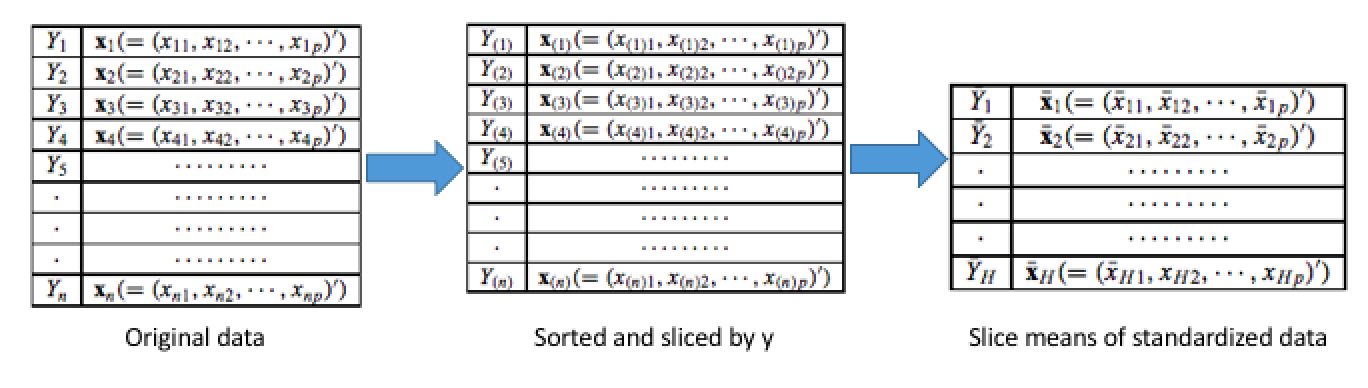
\includegraphics[width=4.16667in]{./pic/slice method.png}
\caption{}
\end{figure}

\begin{enumerate}
\def\labelenumi{\arabic{enumi}.}
\tightlist
\item
  Sort the data based on the response values.\\
\item
  Split data into the slices based on the sorted responses.
\end{enumerate}

\end{frame}

\begin{frame}{Binary response}

Binary response only has two levels, e.g. \(0,1\).

\begin{block}{Limited number of slices}

\begin{itemize}
\tightlist
\item
  Only two slices are available\\
\item
  For SIR, it can only find one direction at most\\
\item
  For SAVE, it also suffers from the limit number of slices
\end{itemize}

\end{block}

\end{frame}

\section{Existing solution}\label{existing-solution}

\begin{frame}{Probability Enhanced (PRE) method (Shin et al. 2014)}

\begin{block}{Main idea}

\begin{itemize}
\tightlist
\item
  \(S_{Y|X} = S_{P(X)}\), \(P(x) = \mathcal{P}(Y = 1|X = x)\) is the
  conditional probability
\item
  \(Y \Rightarrow P(X) \in [0,1]\)
\item
  Weighted Support Vector Machine(WSVM) to estimate the \(\hat{P}(X)\)
\end{itemize}

\end{block}

\begin{block}{Computational time}

\begin{itemize}
\tightlist
\item
  SVM method is sensitive to the number of observation N
\end{itemize}

\end{block}

\end{frame}

\section{Our approach}\label{our-approach}

\begin{frame}{Representative approach}

\begin{block}{Representative}

A Representative is a summary statistic of data points within a cluster:
For \((X_i, Y_i), i \in I_k\) and \(n_k\) is sample size of \(I_k\) \[
  X^*_k = R(X_{1}, \dots, X_{n_k}) = \frac{\sum_i X_i}{n_k},~~ Y^*_k = R(Y_{1}, \dots, Y_{n_k}) = \frac{\sum_i Y_i}{n_k},
\] where \(R\) is the summarizing function.

\end{block}

\begin{block}{Steps}

\begin{enumerate}
\def\labelenumi{\arabic{enumi}.}
\tightlist
\item
  Cluster \((X_1, \dots,X_N)\) into K groups \(I_1, \dots, I_K\),
  e.g.K-means
\item
  Calculate the representatives for each cluster \(I_k\)
\item
  Apply dimension reduction methods on the K representatives
\end{enumerate}

\end{block}

\end{frame}

\begin{frame}{Additional value: Big data solution (N is large)}

\begin{block}{Clustering step}

Clustering step reduced the sample size from \(N\) to \(K\).

\begin{itemize}
\item
  \((Y_1,X_1) \dots (Y_N,X_N) \to (Y^*_{1},X^*_{1}) \dots (Y^*_K,X^*_K)\)
\item
  Note if the data set is too large, we could also use the online
  clustering method.
\end{itemize}

\end{block}

\end{frame}

\begin{frame}{Additional value: Big data solution (N is large)}

\begin{block}{Parallel Algorithm for SIR and SAVE}

\begin{enumerate}
\def\labelenumi{\arabic{enumi}.}
\tightlist
\item
  Split the sliced data into b blocks, \(X_1, \dots X_B\)\\
\item
  Load each block \(X_b\) and calculate the statistics for each block
  such as \(\bar{X}_b, \bar{X}_{hb}, n_{hb}, X^T_{hb}X_{hb}\)\\
\item
  Summary the statistics across the blocks and slices to get the
  candidate matrix \(M_{SIR}, M_{SAVE}\)
\end{enumerate}

\end{block}

\end{frame}

\section{Simulation result}\label{simulation-result}

\begin{frame}{Simulation setup}

\begin{block}{Data generation model: Latent model}

\[
    Y=\left\{
                \begin{array}{ll}
                  0 ~~~f(b_1^TX,b_2^TX, b_3^TX, \epsilon) < 0 \\
                  1 ~~~\text{Otherwise} \\
                \end{array}
      \right. 
\] where

\begin{itemize}
\tightlist
\item
  \(X \in \mathbb{R}^6 \sim N(\mathbf 0, \mathbf I)\)\\
\item
  \(b_i = e_i = (0,\dots, 1,0,\dots,0)^T\), so
  \(b_1^TX = X_1, b_2^TX = X_2, b_3^TX = X_3\)
\item
  \(\epsilon \sim N(0,1)\)
\end{itemize}

\end{block}

\end{frame}

\begin{frame}{Simulation result}

\begin{block}{Performance evaluation}

\begin{enumerate}
\def\labelenumi{\arabic{enumi}.}
\tightlist
\item
  The number of directions of the central space: Hypothesis Test\\
\item
  Difference between a true bias B and an estimated \(\hat{B}\):

  \begin{itemize}
  \tightlist
  \item
    Trace correlation and Frobenius distance
  \end{itemize}
\end{enumerate}

\end{block}

\begin{block}{Result summary}

\begin{itemize}
\tightlist
\item
  The true basis is \((e_1,e_2, e_3)\).\\
\item
  The proposed method is able to recover the whole true central space.
\item
  Other methods can only find part of the central space.
\end{itemize}

\end{block}

\end{frame}

\begin{frame}{Simulation result of SAVE}

\begin{table}[]
\centering
\caption{Simulation result of SAVE}
\resizebox{\textwidth}{!}{%
\begin{tabular}{|c|c|cccc|cccc|}
\hline
\multicolumn{2}{|c|}{\multirow{2}{*}{}}              & \multicolumn{4}{c|}{Original SAVE} & \multicolumn{4}{c|}{Proposed SAVE}                \\ \cline{3-10} 
\multicolumn{2}{|c|}{}                               & \multicolumn{8}{c|}{log n}                                                      \\ \hline
                          & $H_0$ vs $H_1$       & 3      & 4      & 5      & 6      & 3    & 4    & 5             & 6             \\ \hline
\multirow{3}{*}{Power}    & 0D vs \textgreater{}= 1D & 0.9    & 1      & 1      & 1      & 0    & 0.05 & \color{blue}\textbf{1}    & \color{blue}\textbf{1}    \\
                          & 1D vs \textgreater{}= 2D & 0.08   & 0.52   & 0.52   & 0.5    & 0    & 0    & \color{blue}\textbf{1}    & \color{blue}\textbf{1}    \\
                          & 2D vs \textgreater{}= 3D & 0      & 0.05   & 0.06   & 0.06   & 0    & 0    & 0.05          & \color{blue}\textbf{1}    \\ \hline
\multirow{3}{*}{Type-I}   & 3D vs \textgreater{}= 4D & 0      & 0      & 0      & 0.01   & 0    & 0    & 0             & 0.01          \\
                          & 4D vs \textgreater{}= 5D & 0      & 0      & 0      & 0      & 0    & 0    & 0             & 0             \\
                          & 5D vs \textgreater{}= 6D & 0      & 0      & 0      & 0      & 0    & 0    & 0             & 0             \\ \hline
\multirow{2}{*}{Distance} & F                        & 1.33   & 1.2    & 1.21   & 1.19   & 1.71 & 1.03 & \color{blue}\textbf{0.23} & \color{blue}\textbf{0.07} \\
                          & R                        & 0.17   & 0.14   & 0.14   & 0.13   & 0.29 & 0.1  & \color{blue}\textbf{0.01} & \color{blue}\textbf{0}    \\ \hline
\end{tabular}%
}
\end{table}

\end{frame}

\section{Conclusion}\label{conclusion}

\begin{frame}{Conclusion and Future work}

\begin{block}{Conclusion}

\begin{itemize}
\tightlist
\item
  Better recover the central space in binary responses
\item
  Greatly shorten the running time in big data
\end{itemize}

\end{block}

\begin{block}{Future work}

\begin{itemize}
\tightlist
\item
  Investigate optimal the choice of k to achieve the best performance of
  SDR methods.
\end{itemize}

\end{block}

\end{frame}

\begin{frame}{Reference}

\end{frame}

\begin{frame}{Backup}

\begin{examples}

1. Linear regression: $Y = a + b_1^TX + b_2^TX + \epsilon$

2. NonLinear regression: $Y = a + \exp(b_1^TX) + \sin(b_2^TX) + \epsilon$

3. More general: $Y = f(b_1^TX, b_2^TX, \epsilon)$
\end{examples}

\end{frame}

\begin{frame}{Simulation result of SIR}

\begin{table}[]
\centering
\caption{Simulation result of SIR}
\resizebox{\textwidth}{!}{%
\begin{tabular}{|c|c|cccc|cccc|cccc|}
\hline
\multicolumn{2}{|l|}{\multirow{2}{*}{}}              & \multicolumn{4}{c|}{SIR\_Binary} & \multicolumn{4}{c|}{SIR\_PRE} & \multicolumn{4}{c|}{SIR\_R}                 \\ \cline{3-14}
\multicolumn{2}{|l|}{}                               & \multicolumn{12}{c|}{log n}                                                                                    \\ \hline
\multicolumn{1}{|l|}{}    & Direction/Distance       & 3      & 4      & 5      & 6     & 3        & 4    & 5    & 6    & 3    & 4          & 5          & 6          \\
\multirow{3}{*}{Power}    & 0D vs \textgreater{}= 1D & 1      & 1      & 1      & 1     & 1        & .    & .    & .    & 0.75 & \textbf{1} & \textbf{1} & \textbf{1} \\
                          & 1D vs \textgreater{}= 2D & .      & .      & .      & .     & 1        & .    & .    & .    & 0.16 & \textbf{1} & \textbf{1} & \textbf{1} \\
                          & 2D vs \textgreater{}= 3D & .      & .      & .      & .     & 0.96     & .    & .    & .    & 0.01 & 0.01       & 0          & 0.01       \\ \hline
\multirow{3}{*}{Type-I}   & 3D vs \textgreater{}= 4D & .      & .      & .      & .     & 0.5      & .    & .    & .    & 0    & 0          & 0          & 0          \\
                          & 4D vs \textgreater{}= 5D & .      & .      & .      & .     & 0.1      & .    & .    & .    & 0    & 0          & 0          & 0          \\
                          & 5D vs \textgreater{}= 6D & .      & .      & .      & .     & 0.01     & .    & .    & .    & 0    & 0          & 0          & 0          \\ \hline
\multirow{2}{*}{Distance} & F                        & 1.13   & 1.05   & 1.06   & 1.09  & 1.14     & .    & .    & .    & 1.37 & 1.29       & 1.24       & 1.29       \\
                          & R                        & 0.14   & 0.14   & 0.14   & 0.15  & 0.12     & .    & .    & .    & 0.18 & 0.15       & 0.15       & 0.15       \\ \hline
\end{tabular}%
}
\end{table}

Iteration time is 200 and significant level is 0.05

\begin{block}{Performance evaluation}

\begin{enumerate}
\def\labelenumi{\arabic{enumi}.}
\tightlist
\item
  The number of directions of the central space: Hypothesis Test
\item
  Difference between a true bias B and an estimated \(\hat{B}\):

  \begin{itemize}
  \tightlist
  \item
    Trace correlation: \(R = 1 - \frac{1}{k}\sum_{i = 1}^k \rho_i^2\),
    where \(\rho^2_i\) is the i-th eigenvalue of
    \(\hat{B}^TBB^T\hat{B}\).
  \item
    Frobenius distance: \(F = \Vert P_B - P_{\hat{B}}\Vert_F\). where
    \(P_A = A(A^TA)^{-1}A\) and
    \(\Vert A\Vert_F = \sqrt{\sum_i\sum_j a^2_{ij}}\).
  \end{itemize}
\end{enumerate}

\end{block}

\end{frame}

\begin{frame}{Simulation setup}

\begin{block}{Data generation model: Latent model}

\[
    Y=\left\{
                \begin{array}{ll}
                  0 ~~~(b_1^TX)^2*e^{(b_2^TX)}*\sin(b_3^TX) + \epsilon < 0 \\
                  1 ~~~\text{Otherwise} \\
                \end{array}
      \right.
\] where

\begin{itemize}
\tightlist
\item
  \(X \in \mathbb{R}^6 \sim N(\mathbf 0, \mathbf I)\)
\item
  \(b_i = e_i = (0,\dots, 1,0,\dots,0)^T\), so
  \(b_1^TX = X_1, b_2^TX = X_2, b_3^TX = X_3\)
\item
  \(\epsilon \sim N(0,1)\)
\item
  \(P(X) = \Phi((b_1^TX)^2*e^{(b_2^TX)}*\sin(b_3^TX))\), where \(\Phi\)
  is the CDF of standard normal distribution.
\end{itemize}

\end{block}

\end{frame}

\begin{frame}{How it works}

\begin{block}{Main idea}

Y and \(P(X)\) have identical central space: \(S_{Y|X} = S_{P(X)|X}\)

\begin{center}
$Y = f(b_1^TX, \dots, b_d^TX)$
$\Rightarrow$
$\mathcal{P}(Y = 1 |X) = P(X) = P(b_1^TX, \dots, b_d^TX)$
\end{center}

\end{block}

\begin{block}{For the Representative}

\begin{center}
$Y^*_k = \hat{\mathcal{P}}(Y = 1|X_i, i\in I_k) \approx P(b_1^T\bar{X}_k, \dots, b_d^T\bar{X}_k)$
$Y^*_k \rightarrow P(Y=1|X=x_k) \text{ as } N,K,N/K \to \infty$
\end{center}

\hypertarget{refs}{}
\hypertarget{ref-ref7}{}
Cook, R Dennis, and Sanford Weisberg. 1991. ``Discussion of `Sliced
Inverse Regression for Dimension Reduction'.''

\hypertarget{ref-ref9}{}
Kim, Boyoung, and Seung Jun Shin. 2019. ``Principal Weighted Logistic
Regression for Sufficient Dimension Reduction in Binary
Classification.''

\hypertarget{ref-ref6}{}
Li, Ker-Chau. 1991. ``Sliced Inverse Regression for Dimension
Reduction.''

\hypertarget{ref-ref8}{}
Shin, Seung Jun, Yichao Wu, Hao Helen Zhang, and Yufeng Liu. 2014.
``Probability-Enhanced Sufficient Dimension Reduction for Binary
Classification.''

\end{block}

\end{frame}

\end{document}
